\documentclass[11pt]{exam}

\usepackage{amsmath, amssymb, multicol}
\usepackage{graphicx}
\usepackage{textcomp}
\usepackage{chessboard}
\usepackage{tikz}

\def\d{\displaystyle}
\def\b{\mathbf}
\def\R{\mathbf{R}}
\def\Z{\mathbf{Z}}
\def\st{~:~}
\def\bar{\overline}
\def\inv{^{-1}}


\newcommand{\vtx}[2]{node[fill,circle,inner sep=0pt, minimum size=4pt,label=#1:#2]{}}
\newcommand{\va}[1]{\vtx{above}{#1}}
\newcommand{\vb}[1]{\vtx{below}{#1}}
\newcommand{\vr}[1]{\vtx{right}{#1}}
\newcommand{\vl}[1]{\vtx{left}{#1}}
\renewcommand{\v}{\vtx{above}{}}


%\pointname{pts}
\pointsinmargin
\marginpointname{pts}
\addpoints
\pagestyle{head}
%\printanswers

\firstpageheader{Math 228}{\bf Matchings}{April 20, 2015}


\begin{document}

%space for name
%\noindent {\large\bf Name:} \underline{\hspace{2.5in}}
%\vskip 1em

\noindent Given a bipartite graph, a {\em matching} is a subset of the edges for which every vertex belongs to exactly one of the edges.  Our goal in this activity is to discover some criterion for when a bipartite graph has a matching.

\begin{questions}
\question Does the graph below contain a matching?  If so, find one.

\begin{center}
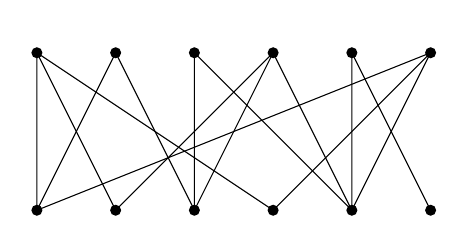
\begin{tikzpicture}
\foreach \x in {0,...,5} {
 \coordinate (a\x) at (\x,0);
 \coordinate (b\x) at (\x,2);
 \draw (a\x) \v (b\x) \v;
 }
\draw (a0) -- (b0) (a0) -- (b1) (a0) -- (b5);
\draw (a1) -- (b0) (a1) -- (b3);
\draw (a2) -- (b1) (a2) -- (b2) (a2) -- (b3);
\draw (a3) -- (b0) (a3) -- (b5);
\draw (a4) -- (b2) (a4) -- (b3) (a4) -- (b4) (a4) -- (b5);
\draw (a5) -- (b4);
\end{tikzpicture}
\end{center}


\question Not all bipartite graphs have matchings.  Draw as many fundamentally different examples of bipartite graphs which do NOT have matchings.  Your goal is to find all the possible obstructions to a graph having a matching.  Write down the {\em necessary} conditions for a graph to have a matching (that is, fill in the blank: If a graph has a matching, then \underline{\hspace{1in}}).  Then ask yourself whether these conditions are sufficient (is it true that if \underline{\hspace{1in}}, then the graph has a matching?).

\newpage

\uplevel{A bipartite graph that doesn't have a matching might still have a {\em partial matching}.  By this we mean a set of edges for which no vertex belongs to more than one edge (but possibly belongs to none).  Every bipartite graph (with at least one edge) has a partial matching, so we can look for the largest partial matching in a graph.}

\question Your ``friend'' claims that she has found the largest partial matching for the graph below (her matching is in bold).  She explains that no other edge can be added, because all the edges not used are connected to matched vertices.  Is she correct?

\begin{center}
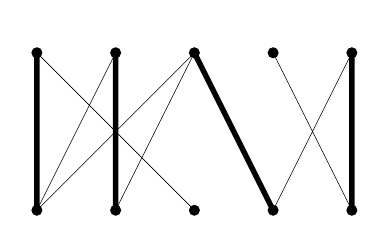
\begin{tikzpicture}
\foreach \x in {0,...,4} {
 \coordinate (a\x) at (\x,0);
 \coordinate (b\x) at (\x,2);
 \draw (a\x) \v (b\x) \v;
 }
 \draw[line width=2pt] (a0) -- (b0) (a1) -- (b1) (a3) -- (b2) (a4) -- (b4);
 \draw[very thin] (a0) -- (b1) (a1) -- (b2) (a2)--(b0)  (a0)--(b2) (a3) -- (b4) (a4) -- (b3);
\end{tikzpicture}
\end{center} 
\vfill

\uplevel{One way you might check to see whether a partial matching is maximal is to construct an {\em alternating path}.  This is a sequence of adjacent edges, which alternate between edges in the matching and edges not in the matching (no edge can be used more than once).  If an alternating path starts and stops with an edge {\em not} in the matching, then it is called an {\em augmenting path}. }

\question Find the largest possible alternating path for the partial matching of your friends graph.  Is it an augmenting path?  How would this help you find a larger matching?

\begin{center}
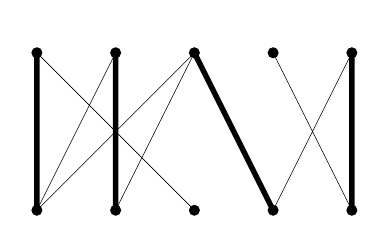
\begin{tikzpicture}
\foreach \x in {0,...,4} {
 \coordinate (a\x) at (\x,0);
 \coordinate (b\x) at (\x,2);
 \draw (a\x) \v (b\x) \v;
 }
 \draw[line width=2pt] (a0) -- (b0) (a1) -- (b1) (a3) -- (b2) (a4) -- (b4);
 \draw[very thin] (a0) -- (b1) (a1) -- (b2) (a2)--(b0) (a0)--(b2) (a3) -- (b4) (a4) -- (b3);
\end{tikzpicture}
\end{center} 
\vfill

\question Find the largest possible alternating path for the partial matching below.  Are there any augmenting paths?  Is the partial matching the largest one that exists in the graph?

\begin{center}
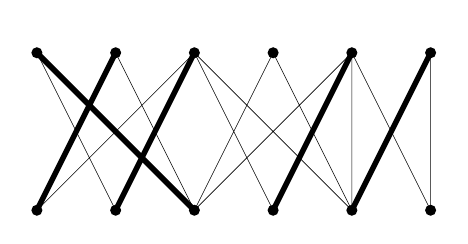
\begin{tikzpicture}
\foreach \x in {0,...,5} {
 \coordinate (a\x) at (\x,0);
 \coordinate (b\x) at (\x,2);
 \draw (a\x) \v (b\x) \v;
 }
 \draw[line width=2pt] (a0) -- (b1) (a1) -- (b2) (a2) -- (b0) (a3) -- (b4) (a4) -- (b5);
 \draw[very thin] (a0) -- (b2) (a1) -- (b0) (a2)--(b1) (a2) -- (b3) (a2) -- (b4) (a3) -- (b2) (a4) -- (b2) (a4)-- (b3) (a4) -- (b4) (a5) -- (b4) (a5)--(b5);
 

\end{tikzpicture}

\end{center} 

\vfill

\end{questions}

\end{document}


